Люди пытались сделать компьютер достаточно давно.
\\Первым (после антикитерского механизма) был \textbf{механизм для суммирования и умножения}. Изобрел его Вильгельм Шиккард (\emph{1592 -- 1635}) в 1623 году.
\\Машина содержала суммирующее и множительное устройства, а также механизм для записи промежуточных результатов. Первый блок -- шестиразрядная суммирующая машина -- представлял собой соединение зубчатых передач. На каждой оси имелись шестерня с десятью зубцами и вспомогательное однозубое колесо -- палец. Палец служил для того, чтобы передавать единицу в следующий разряд (поворачивать шестеренку на десятую часть полного оборота, после того как шестеренка предыдущего разряда сделает такой оборот). При вычитании шестеренки следовало вращать в обратную сторону. Контроль хода вычислений можно было вести при помощи специальных окошек, где появлялись цифры. Для перемножения использовалось устройство, чью главную часть составляли шесть осей с "навернутыми" на них таблицами умножения.
\\Второй арифметической машиной был \textbf{механизм для суммирования и вычитания "Паскал\'ина"}. Изобрел его Блез Паскаль (\emph{1623—1662}) в 1642 году.
\\Машина Паскаля представляла собой механическое устройство в виде ящичка с многочисленными связанными одна с другой шестеренками. Складываемые числа вводились в машину при помощи соответствующего поворота наборных колесиков. На каждое из этих колесиков, соответствовавших одному десятичному разряду числа, были нанесены деления от 0 до 9. При вводе числа, колесики прокручивались до соответствующей цифры. Совершив полный оборот, избыток над цифрой 9 колесико переносило на соседний разряд, сдвигая соседнее колесо на 1 позицию.
\\Следующим был \textbf{арифмометр Лейбница}, умеющий выполнять операции сложения, вычитания, деления и умножения. Изобрел ее Готфрид Вильгельм Лейбниц (\emph{1646 -- 1716}) в 1673 году.
\\Сложение чисел выполнялось при помощи связанных друг с другом колес, так же как на "Паскалине". Добавленная в конструкцию движущаяся часть и специальная рукоятка, позволявшая крутить ступенчатое колесо (в последующих вариантах машины -- цилиндры), позволяли ускорить повторяющиеся операции сложения, при помощи которых выполнялось деление и перемножение чисел. Необходимое число повторных сложений выполнялось автоматически.
\\Прообразом современного компьютера стала \textbf{идея создания универсальной аналитической вычислительной машины}, которую выдвинул Чарльз Бэббидж (\emph{1791 -- 1871}) в 1823 году.
\\В 1822 году Бэббидж построил \textbf{малую разностную машину}. Ее работа была основана на методе конечных разностей. Малая машина была полностью механической и состояла из множества шестеренок и рычагов. В ней использовалась десятичная система счисления. Она оперировала 18--разрядными числами с точностью до восьмого знака после запятой и обеспечивала скорость вычислений 12 членов последовательности в 1 минуту. Малая разностная машина могла считать значения многочленов 7--й степени.
\\И в том же 1822 году Бэббидж задумался о создании \textbf{большой разностной машины} предназначенной для автоматизации вычислений путем аппроксимации функций многочленами и вычисления конечных разностей. Возможность приближенного представления в многочленах логарифмов и тригонометрических функций позволяло бы рассматривать эту машину как довольно универсальный вычислительный прибор. В 1823 году он приступил к проектированию, однако, в 1842 году государство отказалось финансировать проект и машина так и не была достроена. Но для развития вычислительной техники имело значение другое: идея создания аналитической вычислительной машины. В единую логическую схему Бэббидж увязал арифметическое устройство (названное им "мельницей"), регистры памяти, объединенные в единое целое ("склад"), и устройство ввода--вывода, реализованное с помощью перфокарт трех типов. Перфокарты операций переключали машину между режимами сложения, вычитания, деления и умножения. Перфокарты переменных управляли передачей данных из памяти в арифметическое устройство и обратно. Числовые перфокарты могли быть использованы как для ввода данных в машину, так и для сохранения результатов вычислений, если памяти было недостаточно.
\\Следующим этапом в развитии вычислительной техники стал \textbf{электромеханический перфокарточный табулятор для переписи населения}, который изобрел Герман Холлерит (\emph{1860 -- 1929}) в 1880 году.
\\Табуляторы предназначены для автоматической обработки (суммирования и категоризации) числовой и буквенной информации, записанной на перфокартах, с выдачей результатов на бумажную ленту или специальные бланки. Умножение и деление выполнялись методом последовательного многократного сложения и вычитания. Работа табулятора производилась в соответствии с набираемой на коммутационной панели программой.
\\В 1911 году Алексей Николаевич Крылов (\emph{1863 -- 1945}) изобрел \textbf{аналоговый решатель дифференциальных уравнений}. Он интегрировал обыкновенные дифференциальные уравнения.
\\В 1919 году Николай Николаевич Павловский (\emph{1884 -- 1937}) сконструировал \textbf{аналоговую вычислительную машину (АВМ)}. Она была создана для реализации метода исследования природных явлений при помощи аналого--математического моделирования, который разработал Павловский в том же 1919 году.
\\\\Наличие заданного набора исполняемых команд и программ было характерной чертой первых компьютерных систем. Сегодня подобный дизайн применяют с целью упрощения конструкции вычислительного устройства. Так, настольные калькуляторы, в принципе, являются устройствами с фиксированным набором выполняемых программ. Их можно использовать дляматематических расчётов, но невозможно применить для обработки текста и компьютерных игр, для просмотра графическихизображений или видео. Изменение встроенной программы для такого рода устройств требует практически полной их переделки, и в большинстве случаев невозможно. Впрочем, перепрограммирование ранних компьютерных систем всё--таки выполнялось, однако требовало огромного объёма ручной работы по подготовке новой документации, перекоммутации и перестройки блоков и устройств и т. п.
\\\\Всё изменила идея хранения компьютерных программ в общей памяти. Ко времени её появления использование архитектур, основанных на наборах исполняемых инструкций, и представление вычислительного процесса как процесса выполнения инструкций, записанных в программе, чрезвычайно увеличило гибкость вычислительных систем в плане обработки данных. Один и тот же подход к рассмотрению данных и инструкций сделал лёгкой задачу изменения самих программ.

\section{ЭВМ Джона фон Неймана}
\begin{minipage}[l]{3cm}
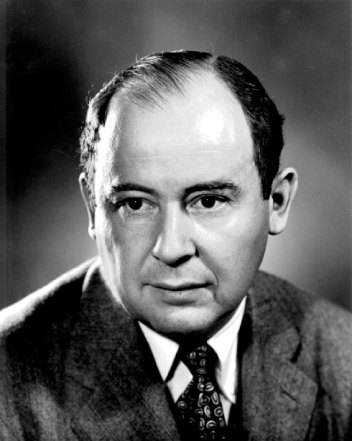
\includegraphics[width=3cm]{9_1}
\begin{center}
\footnotesize{Джон фон Нейман}
\\\footnotesize{$1903 -- 1957$}
\end{center}
\end{minipage}
\hfill
\begin{minipage}[r]{7.5cm}
В 1930--х годах началась разработка архитектуры ЭВМ для военно--морской артиллерии по заказу правительства США. В разработке участвовали Гарвардский университет и Принстонский университет (в том числе и Джон фон Нейман). На рисунке \ref{tag:EVM_von_Neumann} приведена схема ЭВМ, предложенная фон Нейманом.
\end{minipage}
\\
\begin{figure}[h]
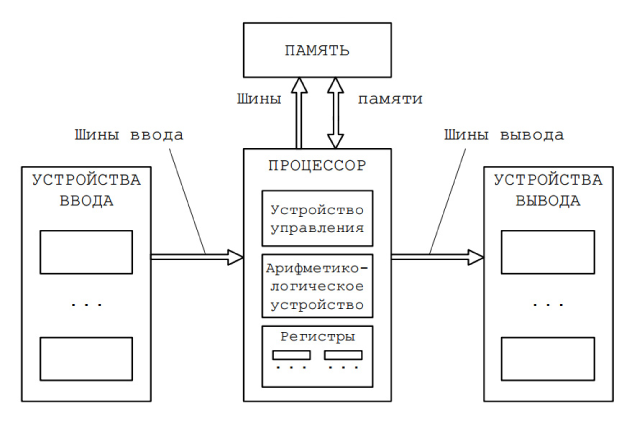
\includegraphics[width=\textwidth]{9_2}
\caption{Структурная схема ЭВМ фон Неймана}
\label{tag:EVM_von_Neumann}
\end{figure}
\subsection{Узлы ЭВМ фон Неймана}
\begin{itemize}
  \item \textbf{Процессор} -- исполнитель машинных инструкций (кода программ), главная часть аппаратного обеспечения ЭВМ. В состав процессора входят:
      \begin{itemize}
        \item устройство управления выборкой команд из памяти и их выполнением;
        \item арифметико--логическое устройство, производящее операции над данными;
        \item регистры, осуществляющие временное хранение данных и состояний процессора;
        \item схемы для управления и связи с подсистемами памяти и ввода--вывода.
      \end{itemize}
  \item \textbf{Устройства ввода} обеспечивают считывание данных с носителей информации и ее представление в форме электрических сигналов, воспринимаемых другими устройствами ЭВМ (процессором или памятью) (мышь, клавиатура, сканер).
  \item \textbf{Устройства вывода} представляют результаты обработки данных в ЭВМ в форме, удобной для визуального восприятия человеком (монитор, принтер) или хранения (DVD--привод, стример). При необходимости они обеспечивают запоминание результатов на носителях, с которых эти результаты могут быть снова введены в ЭВМ для дальнейшей обработки (перфоленты, магнитная лента, магнитный диск и т. п.), или передачу результатов на исполнительные органы управляемого объекта (например, робота). 
  \item \textbf{Устройства ввода--вывода} используются как для хранения данных, так и для их считывания (жесткий диск, флешка).
\end{itemize}
\subsection{Принципы работы архитектуры фон Неймана}
Бёркс, Голдстайн и фон Нейман в 1946 г. в книге "Предварительное рассмотрение логического конструирования электронного вычислительного устройства"  описали принципы:
\begin{itemize}
  \item \textbf{Принцип двоичного кодирования} -- вся информация, поступающая в ЭВМ, кодируется с помощью двоичных сигналов.
  \item \textbf{Принцип однородности памяти} -- программы и данные хранятся в одной и той же памяти. Поэтому ЭВМ не различает, что хранится в данной ячейке памяти -- число, текст или команда. Над командами можно выполнять такие же действия, как и над данными.
  \item \textbf{Принцип адресуемости памяти} -- структурно основная память состоит из пронумерованных ячеек, процессору в произвольный момент времени доступна любая ячейка.
  \item \textbf{Принцип жесткости архитектуры} -- неизменяемость в процессе работы топологии, архитектуры, списка команд.
  \newpage
  \item \textbf{Принцип программного управления}:
  \begin{enumerate}
    \item В начале процессору сообщается адрес первой команды программы (который заносится в специальный \textbf{регистр команд}), после этого программа управляет сама собой.
    \item После выполнения команды процессор увеличивает адрес, хранимый в регистре команд, на длину только что выполненной команды, чтобы получить адрес следующей команды. Так можно выполнить цепочку команд из \textbf{последовательно} расположенных ячеек памяти.
    \item Существуют специальные \textbf{команды переходов}, которые сразу содержат в себе адрес следующей команды. После выполнения таких команд указанный адрес просто заносится в регистр команд. Так можно выполнить цепочку команд из \textbf{непоследовательно} расположенных ячеек памяти.
  \end{enumerate}
\end{itemize}
\section{Классификация архитектур ЭВМ}
\textbf{Архитектура ЭВМ} -- концептуальная структура вычислительной машины, определяющая проведение обработки информации и включающая методы преобразования информации в данные и принципы взаимодействия технических средств и программного обеспечения. \textbf{Архитектурой ЭВМ} определяется, как именно в этой ЭВМ происходит обработка и преобразование данных с учетом конкретных принципов взаимодействия технических средств и программного обеспечения.
\\В 30--х годах правительство США поручило Гарвардскому и Принстонскому университетам разработать архитектуру ЭВМ для военно--морской артиллерии. Победила разработка Принстонского университета (более известная как архитектура фон Неймана, названная так по имени разработчика, первым предоставившего отчет об архитектуре), так как она была проще в реализации. Гарвардская архитектура использовалась советским учёным А. И. Китовым.
\\В настоящее время наибольшее распространение в ЭВМ получили эти 2 типа архитектуры: \emph{принстонская (неймановская)} и \emph{гарвардская}. Обе они выделяют 2 основных узла ЭВМ: центральный процессор и память компьютера. Различие заключается в структуре памяти:
\begin{itemize}
  \item \textbf{Принстонская архитектура}: программы и данные хранятся в одном массиве памяти (микросхеме) и передаются в процессор по одному каналу связи (шине). Проще реализовать (сконструировать), гибкость модификации программ.
  \item \textbf{Гарвардская архитектура}: предусматривает раздельные хранилища и потоки передачи (шины) для команд и данных. Возможность одновременной работы с данными и командами.
\end{itemize}
В более подробное описание, определяющее конкретную архитектуру, также входят: структурная схема ЭВМ, средства и способы доступа к элементам этой структурной схемы, организация и разрядность интерфейсов ЭВМ, набор и доступность регистров, организация памяти и способы её адресации, набор и формат машинных команд процессора, способы представления и форматы данных, правила обработки прерываний. \\
\\По перечисленным признакам и их сочетаниям среди архитектур выделяют:
\begin{enumerate}
  \item \textbf{По разрядности интерфейсов и машинных слов}: 8--, 16--, 32--, 64--, 128--разрядные.
  \item \textbf{По особенностям набора команд и регистров}:
  \begin{itemize}
    \item CISC – Complete Instruction Set Computer
    \item RISC – Restricted (Reduced) Instruction Set Computer
    \item CRISP – Complex--Reduced--Instruction--Set Processor
    \item VLIW – Very Long Instruction Word
  \end{itemize}
  \item \textbf{По количеству вычислителей}: однопроцессорные, многопроцессорные, одноядерные, многоядерные.
  \item \textbf{Многопроцессорные по принципу взаимодействия с памятью}: симметричные многопроцессорные (SMP), масcивно--параллельные (MPP), распределенные.
\end{enumerate}
Существуют следующие архитектуры систем команд (рисунок \ref{commands}):
\begin{itemize}
  \item \textbf{Регистровая архитектура} -- внутри процессора существует специальная память (регистры) для хранения промежуточных результатов.
  \item \textbf{Аккумуляторная архитектура} -- существует один регистр (аккумулятор), в котором хранится результат.
  \item \textbf{Стековая архитектура (MISC } -- Minimal Instruction Set Computer) -- команды не имеют операндов.
\end{itemize}
Типичные операции (сложение и умножение) требуют от любого вычислительного устройства нескольких действий: выборку двух операндов, выбор инструкции и её выполнение, и, наконец, сохранение результата. Идея, предложенная и  реализованная Эйкеном, заключалась в физическом разделении линий передачи команд и данных. В первом компьютере Эйкена «Марк I» для хранения инструкций использовалась перфорированная лента, а для работы с данными — электромеханические регистры. Это позволяло одновременно пересылать и обрабатывать команды и данные, благодаря чему значительно повышалось общее быстродействие.
\\Соответствующая схема реализации доступа к памяти имеет один очевидный недостаток — высокую стоимость. При разделении каналов передачи команд и данных накристалле процессора последний должен иметь почти в два раза больше выводов (так как шины адреса и данных составляют основную часть выводов микропроцессора). Способом решения этой проблемы стала идея использовать общую шину данных и шину адреса для всех внешних данных, а внутри процессора использовать шину данных, шину команд и две шины адреса. Такую концепцию стали называть \textbf { \emph{модифицированной Гарвардской архитектурой.}}
\\Такой подход применяется в современных сигнальных процессорах. Еще дальше по пути уменьшения стоимости пошли при создании однокристалльных ЭВМ -- \textbf{микроконтроллеров}. В них одна шина команд и данных применяется и внутри кристалла.
\\Разделение шин в \emph{модифицированной Гарвардской структуре} осуществляется при помощи раздельных управляющих сигналов: чтения, записи или выбора области памяти.
\\\\В процессоре ограниченное количество команд, как и в языках программирования. И каждую операцию он разбивает на более мелкие и простые микрокоманды. Архитектуры CISC и RISC определяют количество этих микрокоманд. Например, есть всего 10 команд, а все остальные операции можно составить из этих команд -- это архитектура RISC. Или на каждую возможную операцию необходима своя команда -- это будет архитектура CISC. Рассмотрим подробнее.
\subsection{Архитектура CISC}
\textbf{CISC} -- complex instruction set computer -- компьютер с полным набором команд.
\begin{itemize}
  \item много команд;
  \item мало регистров общего назначения (памяти для хранения операндов арифметико--логических инструкций, а также адресов или отдельных компонентов адресов ячеек памяти) (до 32);
  \item разнообразие способов адресации (прямая, косвенная);
  \item много форматов команд различной разрядности;
  \item обработка совмещается с обращением к памяти;
  \item плавающая длина команд.
\end{itemize}
Доля сложных дополнительных команд CISC в общем объеме программ не превышает 10--20\%
. Емкость микропрограммной памяти для поддержании сложных команд может увеличиваться на 60\%
.
\subsection{Архитектура RISC}
\textbf{RISC} -- reduced instruction set computer -- компьютер с сокращенным набором команд.
\begin{itemize}
  \item мало команд (только наиболее часто используемые);
  \item много регистров общего назначения (РОН) (сотни);
  \item есть только две команды обращения к памяти (все остальные команды могут работать только с РОНами);
  \item мало форматов команд и способов указания адресов операндов;
  \item фиксированная длина команд (упрощает обработку).
\end{itemize}
\subsection{Преимущества RISC над CISC}
\begin{enumerate}
  \item Возможность повышения тактовой частоты и упрощения кристалла с высвобождением площади под кэш.
  \item Снижение энергопотребления процессора засчет уменьшения числа транзисторов.
  \item Доля сложных дополнительных команд CISC в общем объеме программ не превышает 10--20\%, а остальные операции похожи на соответствующие аналоги RISC--архитектуры.
  \item Возможность упреждающего выполнения команд.
\end{enumerate}
\textbf{Результат}: большинство современных процессоров являются либо чистыми RISC, либо "CISC--поверх--RISC".
\begin{figure}[h]
\centering
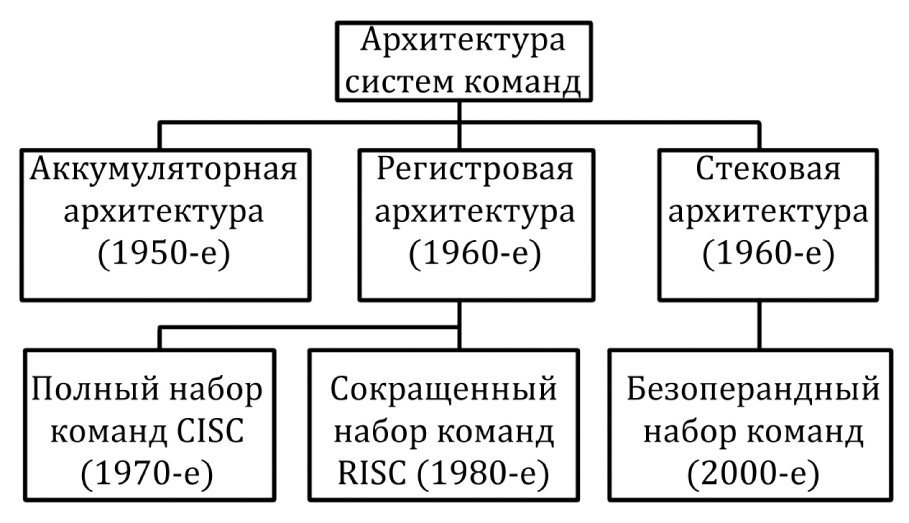
\includegraphics[width=10cm]{9_3}
\caption{Классификация систем команд}
\label{commands}
\end{figure}
\section{Принципы построения ЭВМ}
Перечислим и обощим принципы построения ЭВМ в целом, сформулированные так же фон Нейманом:
\begin{itemize}
  \item наличие единого вычислительного устройства, включающего процессор, средства передачи информации и память;
  \item линейная структура адресации памяти, состоящей из слов фиксированной длины;
  \item двоичная система исчисления;
  \item централизованное последовательное управление, устройство управления выборкой команд из памяти и их выполнением; ;
  \item хранимая программа;
  \item низкий уровень машинного языка;
  \item наличие команд условной и безусловной передачи управления;
  \item АЛУ с представлением чисел в форме с плавающей точкой и производящее операции над данными;;
  \item регистры, осуществляющие временное хранение данных и состояний процессора.
\end{itemize}
\section{Команды процессора}
\begin{figure}[h]
\centering
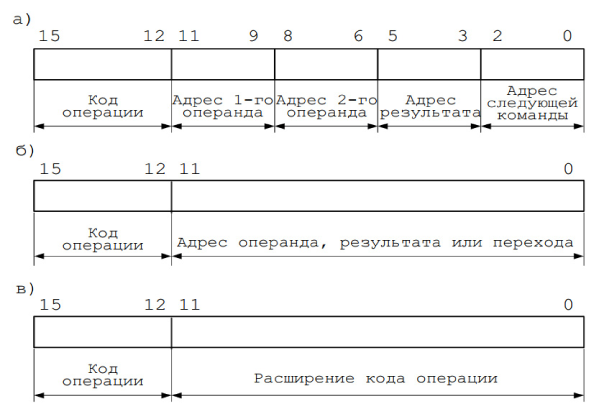
\includegraphics[width=\textwidth]{9_4}
\caption{Форматы команд процессора: а) многоадресная, б) адресная, в) безадресная}
\end{figure}
\begin{center}
  \textbf{Этапы выполнения команд процессором}
\end{center}
Полный цикл выполнения команды может включать в себя следующие этапы:
\begin{itemize}
  \item Вычисление адреса команды (ВАК) -- счетчик команд указывает на некоторую ячейку, содержащую команду;
  \item Выборка команды (ВК) -- обращение к ячейке памяти по адресу, указанному в счетчике команд, считывание команды;
  \item Декодирование команды (ДК) -- процессор распознает, что за команда (сложение, вычитание, переход и так далее);
  \item Вычисление адреса операнда (ВАО) -- если команда адресная, то производится вычисление адреса операнда, который содержит команда;
  \item Выборка операнда (ВО) -- обращение к ячейке памяти по адресу, указанному в команде, считывание операнда;
  \item Выполнение заданной операции (ВЗО);
  \item Запись результата (ЗР).
\end{itemize}
\begin{center}
  \textbf{Конвейерная обработка команд}
\end{center}
При выполнении почти каждой команды, необходимо осуществить 4--7 действий. При выполнении команд последовательно (как это делали старые процессоры) следующая команда будет ждать, пока полностью осуществится первая. Понятно, что можно выполнять команды по принципу конвейера, что существенно увеличит скорость работы.
\begin{figure}[h]
\centering
Пример 5--уровневого конвейера в реальном RISC--процессоре:
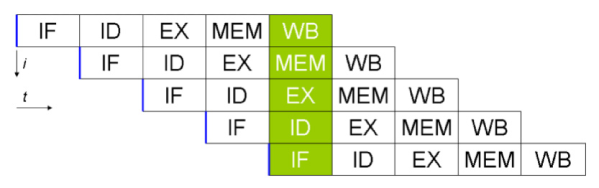
\includegraphics[width=\textwidth]{9_5}
\end{figure}
\begin{description}
  \item[IF] -- ВАК+ВК (вычисление адреса команды и выборка команды);
  \item[ID] -- ДК+ВАО+ВО (декодирование команды, вычисление адреса операнда, выборка операнда);
  \item[EX] -- ВЗО (выполнение заданной операции);
  \item[MEM] -- ЗР (запись результата);
  \item[WB] -- ЗР (запись результата);
\end{description}
Видно, что пока первая команда находится на этапе WB, задействован один узел -- записи результата. Тем временем другой узел -- выполнения заданной операции, может не простаивать, а выполнять третью команду. И таким образом, все отдельные независящие друг от друга узлы, работают одновременно, выполняя этапы разных команд, чем значительно увеличивают производительность.